\documentclass[11pt]{rapport_class}
\usepackage[utf8]{inputenc}
% fonts
\usepackage{lmodern}
\usepackage[T1]{fontenc}

% images, pdfs, urls insertion
\usepackage{hyperref}
\usepackage{graphicx}
\usepackage{pdfpages}
\usepackage{parskip}
\usepackage{xurl}

\title{Plan de projet: Détection de subjectivité dans les news}
\author{IAFA-tigable - Responsable: OLEIWAN Joe \\ Contributeur: DELMOTE Adrien \\ Approbateur: MEUNIER Mortimer}

\date{13/01/2024}

\begin{document}

\maketitle

\begin{abstract}
Dans le cadre du CLEF (Conferences and Labs of the Evaluation Forum) le laboratoire << CheckThat! >> se concentre sur la détection de fake news. Divisé en plusieurs tâches dont la tâche 2 : détecter la subjectivité dans des articles de presse. C'est cette tâche sur laquelle notre équipe de Master informatique (IA et Systèmes embarqués) reprend ce projet collaboratif en ciblant l'utilisation de méthodologies basées sur des Modèles de Langage (LLM) et des dictionnaires. Le document fournit un aperçu détaillé du contexte, des techniques et approches de gestion utilisées, soulignant les objectifs du projet ainsi que son organisation.



\end{abstract}

\smallskip
\begin{motsclefs}
\smallskip
\centerline{-LLM-}
\centerline{-Recherche-}
\centerline{-Méthodes-}
\centerline{-Détection-}
\centerline{-Objectivité-}
\centerline{-Subjectivité-}
\centerline{-Dictionnaire-}
\centerline{-Développement-}
\end{motsclefs}

\tableofcontents

\chapter{Contexte et Objectif}
\section{Contexte}
\qquad Le laboratoire CheckThat! a été organisé pour la 7ème reprise dans le cadre de CLEF 2024. Notre but est d'examiner les travaux précédents et de réaliser la tâche 2 qui consiste à l’identification de la subjectivité. L'objectif de cette tâche est de promouvoir l’intelligence artificielle dans le domaine de la détection de fragments de texte subjectifs depuis des articles de presse ou tweets. La subjectivité est une caractéristique du langage : en prononçant un énoncé le locuteur exprime simultanément sa position, son attitude et ses sentiments à l'égard de celui-ci, laissant ainsi sa propre empreinte. Selon le laboratoire, une phrase est considérée comme subjective si elle contient plusieurs critères tels que :
\begin{itemize}
    \item Rapporter explicitement l'opinion personnelle de son auteur ;
    \item Contenir des expressions sarcastiques ou ironiques ;
    \item Contenir des exhortations ou des auspices personnels ;
    \item Contenir des expressions discriminatoires ou dévalorisantes ;
    \item Contenir des figures de rhétorique explicitement formulées par son auteur pour exprimer son opinion ;
    \item Contenir une conclusion tirée par son auteur en dépit d'informations factuelles insuffisantes ;
    \item Contenir des intensificateurs qui peuvent être attribués à son auteur pour exprimer son opinion ;
\end{itemize}
\begin{tiny}
\href{https://ceur-ws.org/Vol-3370/paper10.pdf}{(cf. On the Definition of Prescriptive Annotation Guidelines for Language-Agnostic Subjectivity Detection)}
\end{tiny}

La tâche propose des corpus composés de 9 530 phrases annotées manuellement, couvrant six langues - arabe, néerlandais, anglais, allemand, italien et turc.

\section{Objectif}
\qquad Il s'agira de développer des modèles basés sur de l'apprentissage automatique. Les modèles utilisés pourront s’appuyer sur des technologies de type  LLM (chatGPT, LangChain, etc.) et/ou sur d'autres modèles de Machine Learning en se basant sur un dictionnaire de textes (ex. : les forêts aléatoires).

Les différents modèles et différentes configurations seront évalués (évaluation de l'efficacité) sur plusieurs jeux de données labelisés.

Fonctionnalité minimale : Un modèle d'apprentissage profond présentant des résultats corrects sur la langue anglaise, un rapport d’évaluation de la prédiction sera rendu ; plusieurs configurations du modèle seront tester

Fonctionnalités complémentaires :
\begin{itemize}
\item D'autres modèles d'apprentissage sur une ou plusieurs langues différentes de l'anglais . 
\end{itemize}


\chapter{Parties prenantes}
\section{UE Management}
\qquad Présentation de l'UE : Faisant partie du programme de première année en Master Informatique, l'Unité d'Enseigement (UE) Management de Projet encadre le projet de quatre mois que nous prenons en charge, elle définit les aspects de gestion du projet et les évalue. 

L'évaluation se fera tout au long de l'UE, avec des travaux que l'on doit aux professeurs de management;
Dates et intitulés des livrables:
\begin{itemize}
    \item Dépôt Rendu kick-off  : 13 janvier 2024
    \item Dépôt Plan projet V1  : 17 février 2024
    \item Dépôt Plan projet V2  : 17 mars 2024
    \item Dépôt Plan project V3 : 14 avril 2024
    \item Dépôt Soutenance finale (Transparent) : avant fin avril 2024
\end{itemize}

\subsection{Communication} 
\qquad La communication avec les responsables de l'UE management ce fait durant les cours de travaux dirigés prévus ainsi qu'à travers un serveur Discord \ref{ discord interne } crée par les responsables pour échanger et poser d'éventuelles questions.


\section{Maître d'ouvrage - Client}
\qquad Le Maître d'ouvrage (MO) est Mme. Josiane Mothe, Professeur en Système d'information, Big Data, Recherche d'information, Exploration d'information et Apprentissage automatique à L'institut de Recherche Informatique de Toulouse (IRIT). Responsable et contributrice à plusieurs projets au cours des années, Mme Mothe nous a proposé ce sujet sur la détection de la subjectivité s'appuyant sur la tâche 2 du CLEF 2023 et 2024 dont le but global est la détection de fake News.

Même si nos modèles répondent aux mêmes critères que ceux demandés pour participer au CLEF 2024, nous ne faisons qu'utiliser les informations et données mises à notre disposition.

\subsection{Communication}
\label{ logs reunions }
\qquad Afin d'assurer une bonne communication avec le client, il a été conclu pendant la réunion de lancement du projet que des réunions de 5 à 15 minutes seront faites en fin de journées sur chacun des deux jours prévus pour le projet dans la semaine, lundi et mardi. Ces réunions rapides nous permettent de tenir la cliente informée de l'avancement du projet et de définir dynamiquement les tâches à effectuer par la suite. Elles sont transcrites dans un fichier log dédié sur le dépôt \href{https://github.com/fghjklm/Projet_M1_CheckThat-/tree/main/log_reunions}{github} Hors des réunions, nous communiquons par mail avec tous les participants en copie (\ref{Controle}). 


\subsection{Capture du besoin}


\qquad Lors d'une réunion de capture du besoin antérieure à celle de lancement du projet et dans nos réunions bi-hebdomadaires, nous écoutons attentivement le client pour saisir ses besoins. Ces échanges sont l'occasion d'ajuster notre compréhension et de préciser le projet. Un tableau récapitulatif est utilisé pour tracer ces besoins, disponible dans le  référentiel de structure de projet \ref{referentiel projet}, assurant que chaque point discuté est bien noté et sera suivi. Ce tableau, régulièrement mis à jour, sert de guide pour le développement et assure que le produit final répondra aux attentes du client.



\section{Assistants maître d'ouvrage}

\qquad Les Assistants à la Maîtrise d'Ouvrage (AMO) M. Julien Contarin et M. Antoine Maîresse, anciens étudiants de M1 ayant fait ce projet en 2023 peuvent avoir le rôle de valider une proposition technique de notre part si besoin, de valider l'organisation du projet, d'accepter la gestion des risques du projet, de proposer des éléments d'assurance et de contrôle qualité ou aussi de nous conseiller dans les exigences à exprimer quant à la maintenabilité ou la pérennité du produit développé, d'assurer la validation des livrables, de valider le référentiel projet.

\subsection{Communication} 

\qquad La communication avec les Assistants maître d'ouvrage est établie à travers les mails échangés avec le client ainsi que dans une section dédié sur le même serveur Discord que nous utilisons interne (\ref{ discord interne }) pour organiser des réunions de gestion projet.



\chapter{Organisation interne}
\section{Organisation du travail}

\qquad Le projet se découpe en deux phases principales que nous abordons chacune avec leur propre méthode de management de projet.

La première phase est la phase de recherche. Nous réalisons un État de l'Art des méthodes utilisées par les équipes de l'année 2023, des recherches effectuées sur la détection automatique de la subjectivité ainsi que l'avancement de la recherche sur les technologies qui pourraient nous être utiles (tel que le prompt engineering). Afin de pouvoir aisément diriger nos recherches, nous adoptons ici une méthode KanBan avec des discussions internes et avec le client de manière régulière.

Après avoir effectué le choix de technologie, nous basculeront vers une méthode AGILE pour mieux convenir aux besoins de management dans la phase de développement. \ref{referentiel projet}\\

\begin{center}
    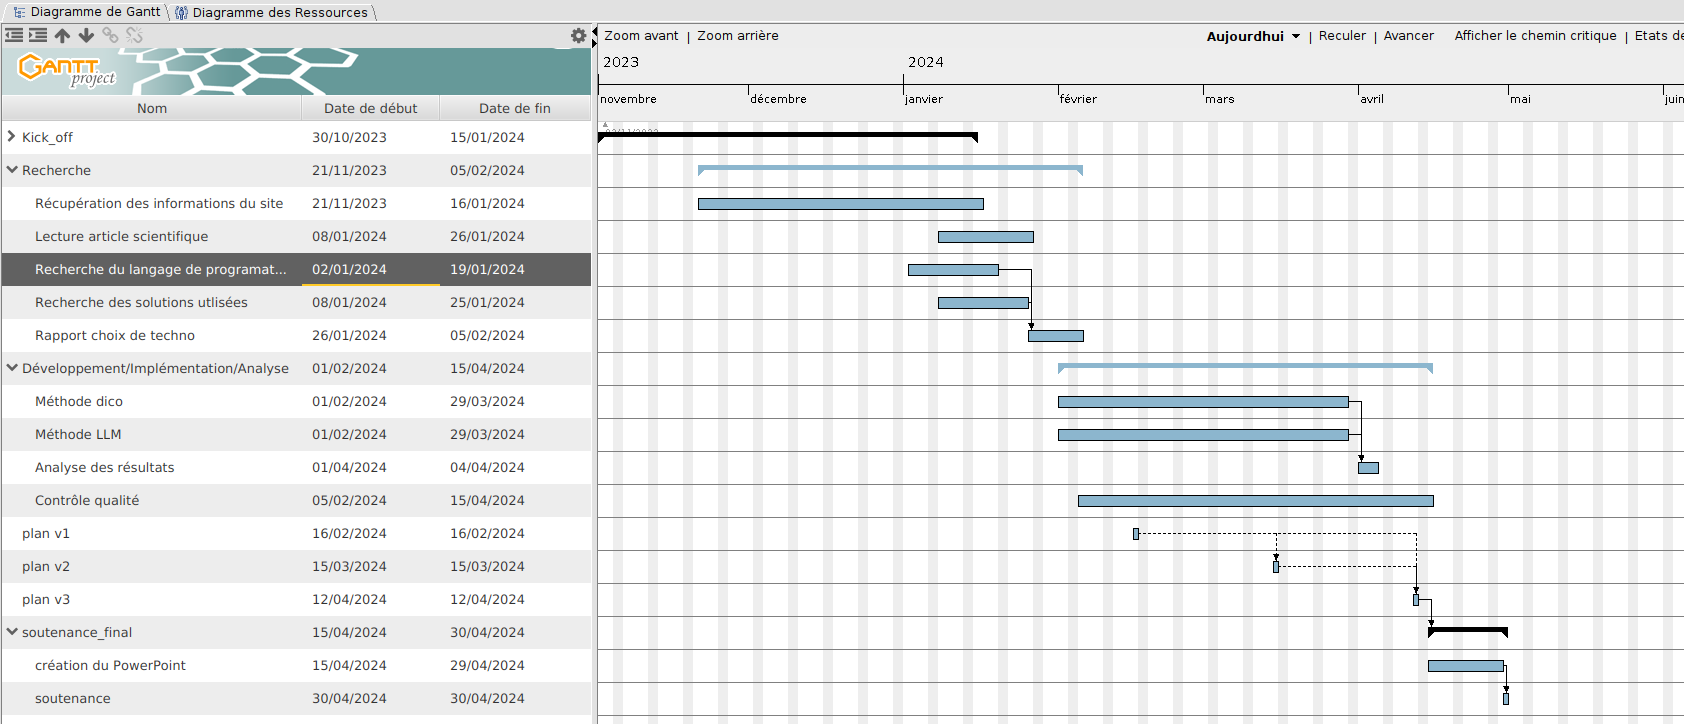
\includegraphics[height= 5cm]{gantt_initiale.png}\\
    \begin{tiny}
        Capture d'écran du Gantt initiale sur GanttProject
    \end{tiny}
\end{center}
Nous avons aussi réaliser un Gantt initiale, dans le but de pouvoir nous organiser et avoir un "squelette" sur les tâches que nous devons accomplir ainsi que le temps que nous estimons. Ce planning ainsi que les plannings courants (évolutif) sont disponible dans le référentiel de structure du projet \ref{referentiel projet}.

\section{Communication}
\label{ discord interne }
\qquad Afin de faciliter la communication interne, nous utilisons la plateforme de messagerie instantanée: Discord. L'objectif de Discord est de nous permettre de communiquer rapidement et de se partager des documents avant validation. Pour s'assurer que le serveur Discord reste organisé, chaque membre du groupe a les permissions nécessaires afin de créer, remanier ou supprimer les canaux de discussion.
Au besoin, selon les tâches en cours, nous nous rassemblons en présentiel pour collaborer.


\section{Suivi des tâches}
\qquad Nous utilisons un outil de gestion de projet en ligne inspiré de la méthode KanBan : Trello. Il nous permet d’indiquer les différentes tâches à faire, les tâches en cours ainsi que les tâches finies, afin d’avoir un réel suivi sur le projet pour l’ensemble des membres du groupe. Le Trello nous sert aussi à regrouper tous les points à aborder et les informations importantes transmises lors des réunions, avant de les transcrire proprement dans les comptes-rendus de réunions \ref{ logs reunions  }.

Référentiel de structure projet : Nous établissons un document Excel qui permet de sauvegarder la structuration de projet au niveau OBS (Organisation Breakdown Structure), PBS (Project Breakdown Structure), WBS (Work Breakdown Structure), diagramme de Gantt intial et un diagramme de gantt que nous mettons à jour au fur et à mesure des besoins.

\section{Gestion des ressources et de la production}
\qquad Pour gérer nos ressources et nos productions, nous utilisons un système de contrôle de version distribué populaire : github. Nous déposons dans ce dépôt tous les documents validés d'après nos règles de qualité (cf.\ref{Controle}). La gestion automatique des versions fournie par git et github nous permettent de pouvoir constamment accéder aux versions antérieures de chaque document. Le dépôt est visible publiquement afin de permettre aux parties prenantes de pouvoir consulter les ressources qui les intéressent.

Lien github : \url{https://github.com/fghjklm/Projet_M1_CheckThat-}

En parallèle, nous utilisons le logiciel Zotero afin de regrouper tous les articles potentiellement liés à nos objectifs. Nous effectuons des synthèses de ceux nous semblant les plus pertinents qui se retrouvent dans le dépôt \href{https://github.com/fghjklm/Projet_M1_CheckThat-/tree/main/articles}{git}.


\chapter{Phase de Recherche}
\section{Modèles et résultats des équipes de CLEF 2023}
CLEF : Conference and Labs of the Evaluation Forum.\\
\vspace{0mm}
\qquad L'accès aux rapports des équipes de CLEF 2023 est une opportunité de taille dans la réalisation de notre projet. Nous explorons les méthodes ayant été utilisées et essayons d'en extraire les informations utiles : les modèles, méthodes de fine-tuning ou les raisons des mauvais résultats de certaines équipes.

\section{État de l'Art de la détection automatique de la subjectivité}
\qquad Nous effectuons également un \href{https://github.com/fghjklm/Projet_M1_CheckThat-/tree/main/articles}{état de l'art de la détection automatique de la subjectivité} afin de découvrir s'il existe des pistes différentes de celles explorées par les équipes de l'an dernier.



\section{Avancement de la recherche sur le prompt engineering}
\qquad Lors de la phase développement, un élément essentiel dont nous aurons besoin est le prompt engineering. Nous effectuons des recherches afin de trouver les méthodes les plus efficaces utilisées sur des travaux de recherche précédents. L'objectif est de perfectionner les requêtes que nous formulerons au LLM sélectionné dans \href{https://github.com/fghjklm/Projet_M1_CheckThat-/tree/main/choix_techno}{le choix de technologie}.




\chapter{Phase de développement}
\centerline{En construction - à établir dans une version future du Plan Projet.}




\chapter{Contrôle Qualité}
\label{Controle}
\qquad Dans le but de mener à bien le projet, nous définissons plusieurs objectifs de qualité, tant sur la qualité des livrables que sur la qualité de notre organisation générale. 

\section{Clarté de communication avec les parties prenantes}
\begin{enumerate}
    \item Au préalable des réunions, résumer au maximum les informations obtenues dans la journée.
    \item Lors des réunions, ne pas perdre de temps sur le son/écran fonctionnant mal. S'il y a un souci, les autres participants l'indiqueront.
    \item Lors des réunions, un seul interlocuteur de l'équipe résume l'ensemble et la personne concernée détaille son point si demandé/nécessaire.
    \item Le trello sert de référentiel pour le travail à effectuer, il doit être mis à jour avant ou après chaque réunion.
    \item S'il y a des remarques ou question à poser au client, elles doivent apparaître sur le Trello dans l'onglet adéquat.
    \item Template de compte-rendus de réunion à suivre.
    \item Les mails doivent avoir une syntaxe [ IAFA-tigable ][Check that! Subjectivity] objet et en copie tout le monde ( CLient AMO et l'équipe).
\end{enumerate}

\section{Accessibilité des informations récoltées}
\begin{enumerate}
    \item Tous les articles lus, même de manière incomplète, doivent apparaître sur Zotero.
    \item Tout article utile au projet doit être synthétisé (au moins les informations utiles).
    \item Le github contient la liste des articles utiles mais pas encore synthétisés.
    \item Toutes les synthèses d'article doivent être dans le github.
    \item Nom des commit github: écrits en minuscules et underscore à la place des espaces.
    \item Clarté des synthèses :
    \begin{enumerate}
        \item La synthèse doit suivre le Template de synthèse de lecture de papiers de recherche (Template différent pour les compte-rendus des équipes 2023).
        \item Nom des synthèses des compte-rendus des équipes 2023: "nom équipe" "quelques mots clef (2/3)" "synthèse".
        \item Nom des synthèses d'articles scientifiques: "sujet article" "mots clef (2/3)" "synthèse".
        \item La synthèse d'un document lu doit contenir en haut de page le nom du lecteur afin de savoir à qui s'adresser pour obtenir plus d'informations.
        \item Si possible, indiquer le paragraphe du document contenant l'information notée.
        \item Le lien vers l'article doit apparaît tout en haut de la synthèse.
    \end{enumerate}
\end{enumerate}

\section{Accessibilité des travaux effectués}
\begin{enumerate}
    \item Le discord ne sert qu'à communiquer à un instantanément ou à montrer un document avant qu'il soit validé. Après validation, il faut transférer les ressources dans l'endroit adéquat du github.
    \item Pour les documents nécessitant un logiciel (par exemple le gantt): le format de base doit être présent sur le github pour pouvoir le modifier aisément mais également une image (png ou jpeg) afin que tous puissent le consulter facilement.
    \item Règles du github (En construction).
    \item Nom des commit github: écrits en minuscules et underscore à la place des espaces.
\end{enumerate}
\section{Clarté des livrables d'UE}
\begin{enumerate}
    \item Cohérence des différentes parties du plan de projet.
    \item Division correcte des parties du plan de projet.
    \item Garder une trace des révisions effectuées et des anciennes versions des documents importants : 
    \item Plan projet écrit au présent.
    \item Repasser une seconde fois par une personne différente, sur les documents écrits pour vérifier les fautes d'orthographe.
    \item Les documents suivants doivent être validés par au moins deux personnes qui ne les as pas écrites avant d'apparaître sur le github: Gantt, compte-rendus de réunion.
    \item Les documents suivants doivent être validés par tous à chaque version avant d'apparaître sur le github: plan de projet, Référentiel de structure de projet.
    \item La validation consiste en une réaction check vert sur Discord
\end{enumerate}
\section{Clarté des livrables auprès du client}
\begin{enumerate}
    \item Repasser une seconde fois par une personne différente, sur les documents écrits pour vérifier les fautes d'orthographe.
    \item Les documents suivants doivent être validés par au moins deux personnes qui ne les as pas écrites avant d'apparaitre sur le github: Gantt, compte-rendus de réunion.
    \item Les documents suivants doivent être validés par tous à chaque version avant d'apparaître sur le github:choix de technologie, les rapports intermédiaires de développement à rendre,
    \item La validation consiste en une réaction check vert sur Discord dans le cas d'une conformité totale.
\end{enumerate}

\chapter{ État actuel du projet}
\qquad Dans cette section, nous présentons des liens vers les ressources actuelles du projet, structurées sur un dépôt github (cliquez sur les bouttons représentés par <- Boutton ->), vous y trouverez le référentiel de structure du projet, le diagramme de Gantt, les différentes versions de ce document et les avancements de la recherche et du développement.

\section{Référentiel de structure du projet}
\label{referentiel projet}
\qquad Le référentiel du plan projet, comprenant l'organisation de la structure à travers l'Organisation Breakdown Structure (OBS), le Project Breakdown Structure (PBS), le Work Breakdown Structure (WBS), est accessible ici :
\href{https://github.com/fghjklm/Projet_M1_CheckThat-/tree/main/referentiel_projet}{<- Référentiel projet ->}

\section{Versions du Plan Projet}
\qquad Les autres versions du Plan Projet sont accessibles ici :
\href{https://github.com/fghjklm/Projet_M1_CheckThat-/tree/main/plan_projet}{<- Plan Projet ->}

\section{Diagramme de Gantt actuel}
\qquad Vous pouvez consulter le diagramme de Gantt actuel pour suivre l'évolution du projet en utilisant ce lien :
\href{https://github.com/fghjklm/Projet_M1_CheckThat-/tree/main/gantt}{<- Gantt ->}

\section{Avancement de la recherche}
\qquad Pour voir les progrès de notre recherche, veuillez consulter ce dossier :
\href{https://github.com/fghjklm/Projet_M1_CheckThat-/tree/main/articles}{<- La Recherche ->}

\section{Avancement du développement}
\qquad L'avancement du développement du projet est disponible dans le dossier suivant :
\href{https://github.com/fghjklm/Projet_M1_CheckThat-/tree/main/code}{<- Le développement ->}

\section{Check list d'autoévaluation PMP}
\qquad Pour voir la check list d'autoévaluation, veuillez consultez ce dossier : 
\href{https://github.com/fghjklm/Projet_M1_CheckThat-/tree/main/plan_projet}{<- CheckList ->}

\section{Autres ressources}
\qquad Toutes les autres ressources liées au projet, tels que les rapports intermédiaires, les documents de conception, et les résultats des tests, sont également disponibles dans notre page GitHub.


\chapter{ Bilan}
\centerline{En construction - à établir dans la version 3 du Plan Projet.}
\end{document}